\documentclass{report}
\usepackage{graphicx}
\usepackage{url}
\usepackage{multirow}
\usepackage{listings}
\lstset{
basicstyle=\small\ttfamily,
columns=flexible,
breaklines=true
}

\author{
    \begin{tabular}{l l}
        \textbf{Submitted By} & \textbf{Sumbitted To} \\
        Aadarsha Dhakal & Asst.Prof.Rajani Chulyado \\
        \multirow{2}{*}{Roll No: 12}  & Department of Computer \\
                                      & Science and Engineering
    \end{tabular}
}
\title{

\includegraphics[width=0.5\textwidth]{kulogo}\\[1cm]
\LARGE{KATHMANDU UNIVERSITY}\\
\large{\textsc{Department of Computer Science and Engineering}}\\[1cm]
\textsc{\large Database Management System}\\
\large{COMP 232}\\[2cm]
\hrule
\vspace{0.5cm}
Lab 2 Report
\vspace{0.5cm}
\hrule
}
\date{
    \vspace{1cm}
    Date: 20-02-2022
}


\begin{document}
\maketitle
\tableofcontents
\listoffigures
\newpage

\begin{figure}
\centering
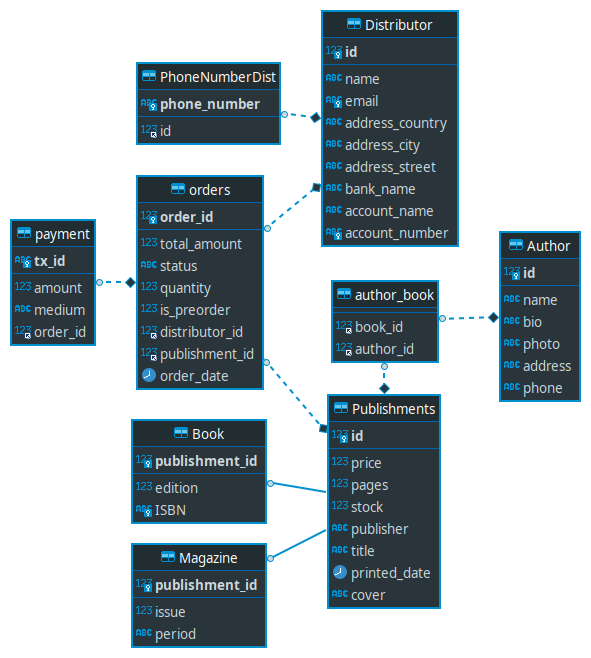
\includegraphics[width=\textwidth]{erdiagram}
\caption{Database ER Diagram}
\end{figure}

\chapter{DDL Scripts}
\section{Creating the tables}
\begin{verse}
    \lstinputlisting{creating_tables.sql}
\end{verse}
\section{Populating data}
\begin{verse}
    \lstinputlisting{populating_data.sql}
\end{verse}

\section{Queries}

\subsection{Find the name of all published books.}
\subsection{Find the name of all books published before 2000.}
\subsection{Get the details of the books written by a particular author.}
\subsection{Find the name of all weekly publications. }
\subsection{Find the name of pre-ordered books.}
\subsection{Get the details of all publications with the name starting with an 'A'.}
\subsection{Find all the orders for a particular book. The result must be sorted based on the order date. }

\chapter{Pattern Matching}


\end{document}
